\chapter{Design}

\section{Mapping between physical world and aggregate abstraction}

The mapping between physical world and protelis program, \autoref{fig:mapping}, is the following:
\begin{itemize}
    \item every sensor is a node of protelis program
    \item every user is a node of protelis program
    \item every user destination is a node of protelis program
\end{itemize}

\begin{figure}[h]
    \centering
    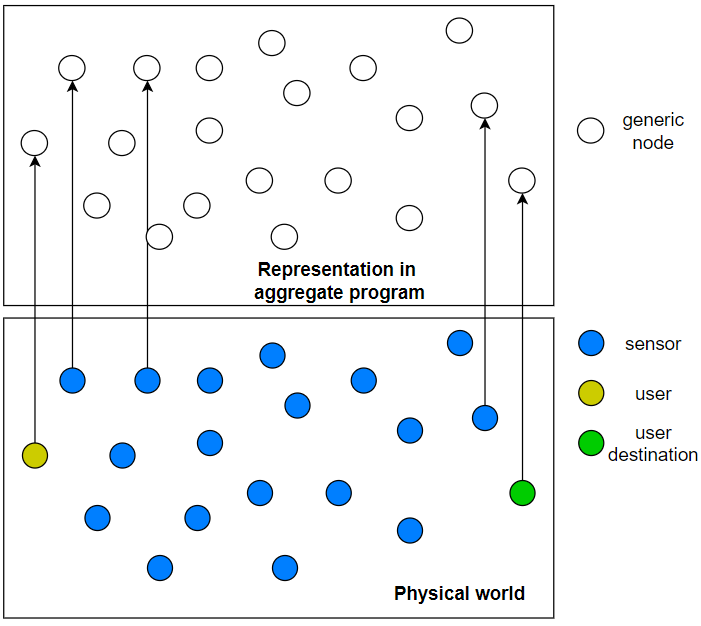
\includegraphics{images/mapping_physicalWorld_ac.png}
    \caption{Mapping between physical world and aggregate abstraction}
    \label{fig:mapping}
\end{figure}
This three different kind of entity will be Protelis nodes with different capabilities, and each nodes will be connected to the other with a proximity based network model. 
Every node of the protelis program retrieves the data of the physical counterpart from the MQTT server where it publishes them.

\clearpage
\section{Design Protelis backend}
\subsection{Entity model}
In this application we have three different typology of nodes with different capabilities:
\begin{itemize}
    \item \textit{SensorNode} $\rightarrow$ represent a sensor device with sensing capabilities
    \item \textit{UserNode} $\rightarrow$ represent a user device. It can require a path and it is also possible that it can have sensing capabilities
    \item \textit{DestinationNode} $\rightarrow$ represent the destination of the required path. It \textbf{don't} have physical counterpart.
\end{itemize}
The model of this kind of entities is present in \autoref{fig:node}
\begin{figure}[h]
    \centering
    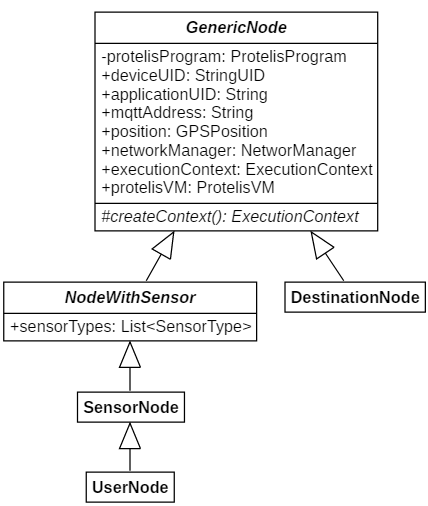
\includegraphics[scale=0.9]{images/nodeModel.png}
    \caption{Model of different types of nodes}
    \label{fig:node}
\end{figure}

\subsection{Execution Context}
The modeling of the execution context for \textit{SensorNode} and \textit{UserNode} is presented in \autoref{fig:execModel_a}.

\begin{figure}[h]
    \centering
    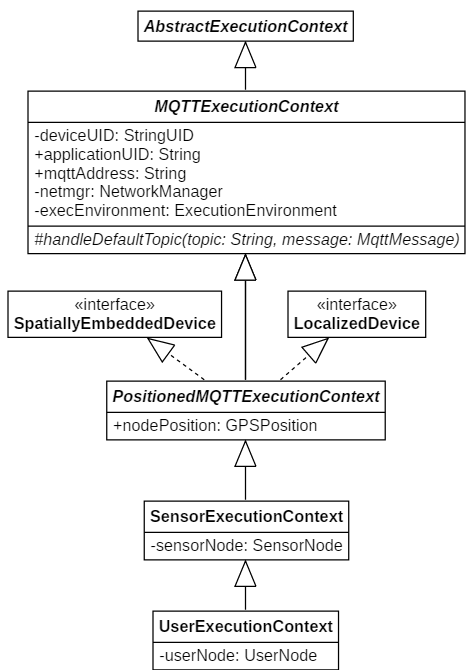
\includegraphics[scale=0.9]{images/execContextModel_v3a.png}
    \caption{Model of execution context for for \textit{SensorNode} and \textit{UserNode}}
    \label{fig:execModel_a}
\end{figure}

\begin{itemize}
    \item \textit{MQTTExecutionContext} $\rightarrow$ encapsulates the subscription to the MQTT server where the physical counterpart publish its data
    \item \textit{PositionedMQTTExecutionContext} $\rightarrow$ implements all the methods of the two interfaces for spatial capabilities
    \item \textit{SensorExecutionContext} $\rightarrow$ manage sensed value like: device position and air quality sensor value. 
    \item \textit{UserExecutionContext} $\rightarrow$ manage the request of route generation and send it to the user device
\end{itemize}

\textit{DestinationNode} doesn't require to communicate via MQTT with the physical counterpart (because there is not any physical counterpart), so its ExecutionContext is more simple and implements only the two interfaces for spatial capabilities. Its UML schema is presented in \autoref{fig:execModel_b}

\begin{figure}[h]
    \centering
    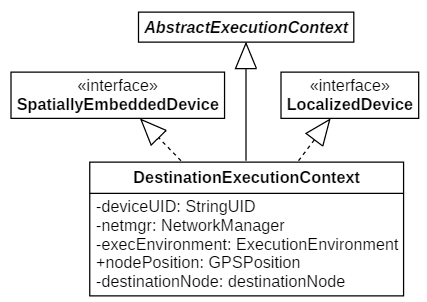
\includegraphics[scale=0.9]{images/execContextModel_v2b.png}
    \caption{Model of execution context for for \textit{DestinationNode}}
    \label{fig:execModel_b}
\end{figure}

\subsection{Network Manager}
Currently the Network Manager is based on MQTT as it is already used for the Execution context.

\section{Model of DingNet simulator}

The model of the environment of simulation is presented in \autoref{fig:envDing}. It is composed from:
\begin{itemize}
    \item \textit{Environment} $\rightarrow$ represent the environment of the simulation. It contains: a reference to all the entity, geographical information and the global clock to share it with the other entity.
    % \todo[inline]{the clock maybe should not be here, but this modification is not a priority}
    \item \textit{Mote} $\rightarrow$ represent a device that can send only packets with data sensed from its sensors
    \item \textit{UserMote} $\rightarrow$ represent the user device that can send packets with sensed data but also packets with the request for a route.
\end{itemize}
% \todo[inline]{I think the other entities have good name and they don't require an explanation for the moment. If it is not so, I will add a description also for the other entities}
\begin{figure}[h]
    \centering
    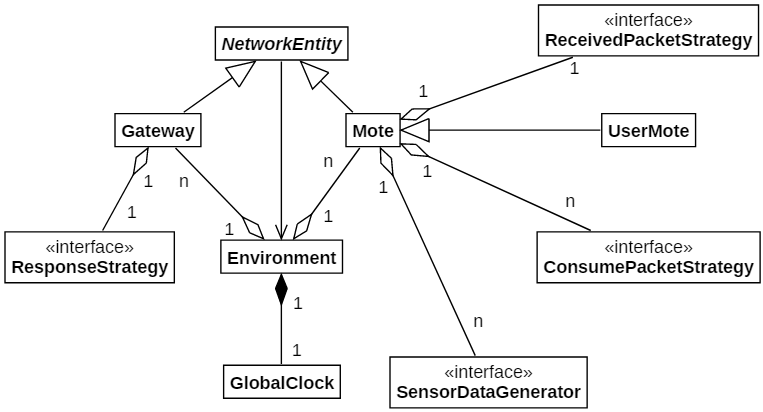
\includegraphics[scale=0.9]{images/envDing.png}
    \caption{Model of the DingNet environment}
    \label{fig:envDing}
\end{figure}

In \autoref{fig:loraDing} is presented the model of the LoRa transmission and of a LoRa packet.
% \todo[inline]{As above, I think the entities have good name and they don't require an explanation for the moment. If it is not so, I will add a description for the entities}

\begin{figure}[h]
    \centering
    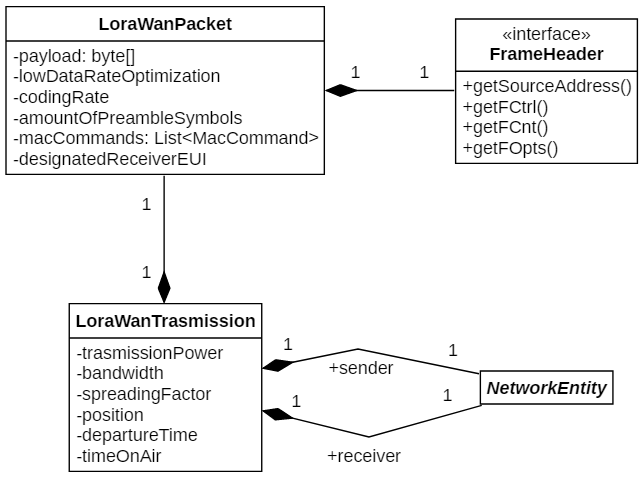
\includegraphics[scale=0.9]{images/loraDing.png}
    \caption{Model of a LoRa transmission and of a LoRa packet}
    \label{fig:loraDing}
\end{figure}